\documentclass [a4paper,12pt,utf8]{report}
\usepackage [francais]{babel}
\usepackage[utf8]{inputenc}
\usepackage[T1]{fontenc}
\usepackage{url}
\usepackage{graphicx}
\usepackage{rotating}

\begin{document}

\begin{titlepage}
\begin{center}
{\bf Université Sciences et Technologies - Bordeaux 1} \vspace{0.5cm}\\

{\bf {\large Master 1 Informatique }}\\
{ \emph{Projet de programmation}}\\\vspace{5cm}



{\huge{\bf Génération procédurale de terrains et de planètes}}\\\vspace{1cm}

{\large{\bf{Rapport No.3:}}}\vspace{1cm}

{\large\bf\it\rm Architecture de la bibliothèque
}\vspace{1cm}


\end{center}


\hspace{1cm}\textbf{Réalisé par:}

\hspace{1cm}{Simon CAULE}

\hspace{1cm}{Pierre HUCHANT}

\hspace{1cm}{Solène JOLLY}

\hspace{1cm}{Adrien LAMOUREUX}\\


\hspace{1cm}\textbf{Encadrés par:} Adrien BOUSSICAULT\\

\hspace{1cm}\textbf{Client:} Emmanuel FLEURY\\

\hspace{1cm}\textbf{Version:} 2.0\\

\hspace{1cm}\textbf{Date:} 01/03/2014\\

\end{titlepage}

\tableofcontents

\chapter{Architecture globale}

Le projet consiste à construire une bibliothèque permettant de générer plusieurs
types de cartes d'élévations (planes, sphériques) à l'aide de diverses
méthodes (fractales, bruits), de générer leurs texture associées, de les
importer et exporter dans différents formats et enfin de les visualiser.

La figure \ref{fig:class-diagram} présente l'architecture que nous avons imaginé,
elle sera décrite plus en détails dans le chapitre suivant.

\begin{sidewaysfigure}
  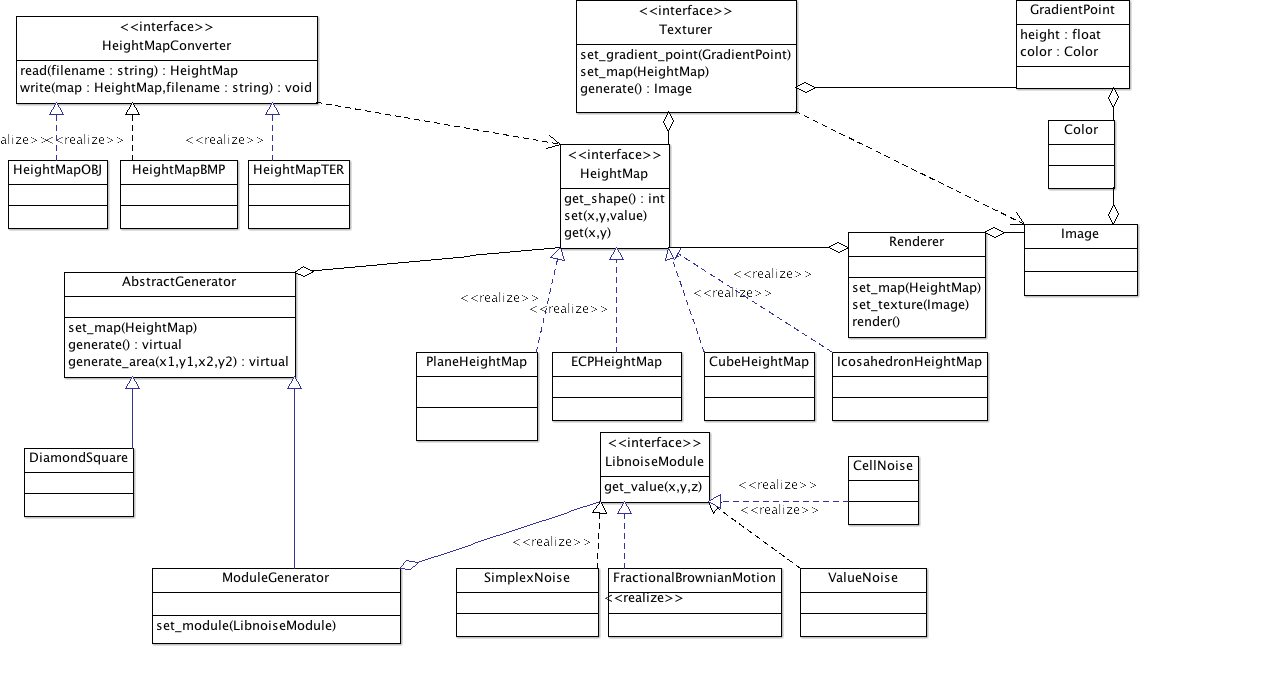
\includegraphics[width=28cm]{resources/class-diagram.png}
        \caption{Diagramme de classe}
        \label{fig:class-diagram}
\end{sidewaysfigure}

\chapter{Descriptions des composants}

\section{Les cartes d'élévations}

Nous avons décidé d'implémenter quatre types de cartes d'élévations :\\

\begin{itemize}
\item \textbf{PlaneHeightMap} : cette classe implémente une carte d'élévations plane.
\item \textbf{ECPHeightMap} : cette classe implémente une carte d'élévations sphérique
sous forme de planisphère.
\item \textbf{CubeHeightMap} : cette classe implémente une carte d'élévations sphérique
sous forme de cube.
\item \textbf{IcosahedronHeightMap} : cette classe implémente une carte d'élévations
sphérique sous forme d'icosaèdre.\\
\end{itemize}

Ces classes implémentent toutes l'interface \textbf{HeightMap} qui permet de
connaître la forme d'une carte (méthode \emph{get\_shape()}), et d'assigner et de
récupérer l'élévation pour des coordonnées données.

\section{La génération des élévations}
La classe \textbf{AbstractGenerator} est une classe abstraite qui permet
d'assigner à un générateur une carte, et qui déclare les méthodes abstraites
\emph{generate\_area()} et \emph{generate()} permettant de générer les
élévations sur toute la carte ou bien seulement sur une zone donnée.\\

De cette classe héritent deux classes, \textbf{DiamondSquare} qui implémente
l'algorithme Diamant-Carré et \textbf{ModuleGenerator}.\\

La classe \textbf{ModuleGenerator} permet de générer une carte en lui assignant
un module de la librairie Libnoise. Nous pouvons donc utiliser tous les modules
de Libnoise et conserver ainsi le mécanisme de communication entres les
différents modules de générations que cette librairie propose.\\

Par conséquent les classes \textbf{SimplexNoise}, \textbf{ValueNoise},
\textbf{CellNoise} et \textbf{FractionalBrownianMotion} devront toutes hériter
de la classe \textbf{noise::module} de Libnoise (appelée \textbf{LibnoiseModule} sur
la figure \ref{fig:class-diagram}).

\section{La génération de texture}
La génération de texture se fera à l'aide de la classe \textbf{Texturer} qui
permet d'assigner une carte d'élévations, des \textbf{GradientPoint} et de
générer une image (méthode \emph{generate()}).\\

La classe \textbf{GradientPoint} n'est rien d'autre que l'association d'une
couleur et d'une élévation. Ainsi après avoir ajouté plusieurs
\textbf{GradientPoint} à un \textbf{Texturer}, la couleur de chaque pixel de la
texture générée sera obtenu en fonction l'élévation du point correspondant
sur la carte et de l'interpolation de couleur entre les différents
\textbf{GradientPoint}.

\section{L'importation et l'exportation des cartes.}
Trois classes permettent d'importer et d'exporter des carte d'élévations sous
format TER (Terragen), OBJ (Blender) ou BMP. Ces trois classes implémentent
toute l'interface \textbf{HeightMapConverter} qui déclare les méthodes
\emph{read()} et \emph{write()} pour l'importation et l'exportation.

\section{La visualisation}
La classe \textbf{Renderer} permettra de visualiser une carte grâce à la méthode
\emph{render()}, à condition de lui avoir préalablement assigné une carte
d'élévation et une texture.

Il est évident que l'implémentation du visualisateur sera bien plus complexe et
ne sera pas limité à une seule classe cependant nous n'avons pas encore eu le
temps de réaliser complètement l'architecture de celui-ci.

\chapter{Diagramme de Séquence}
\begin{figure}[h!]

        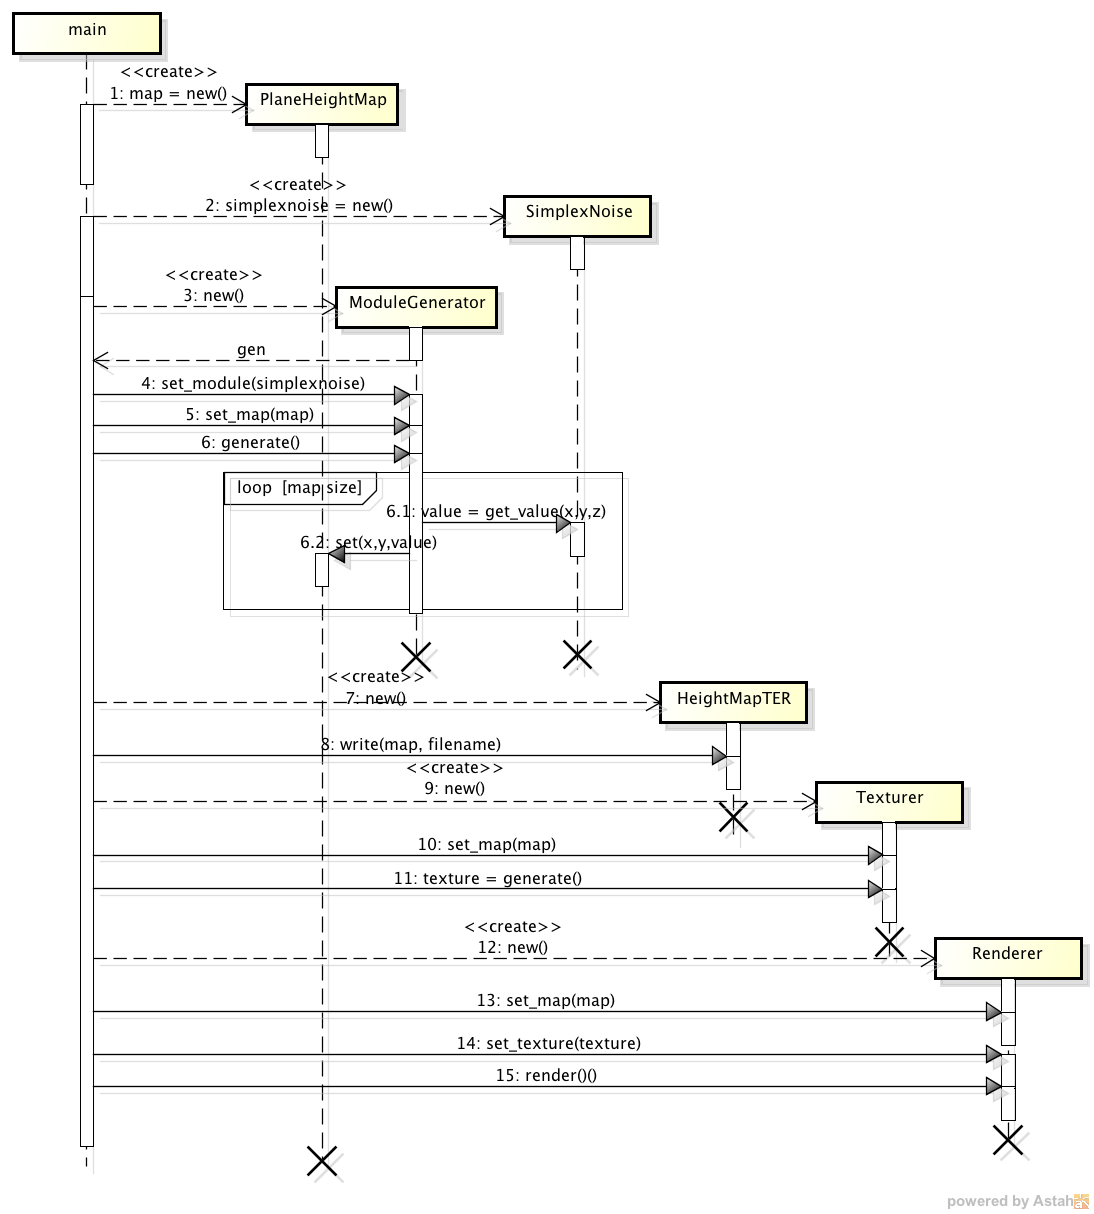
\includegraphics[width=15cm]{resources/sequence-diagram.png}
        \caption{Diagramme de séquence}

\end{figure}



\end{document}
